\documentclass[oneside,a4paper,12pt]{article}
\usepackage{graphicx}
\usepackage[section]{placeins}
\usepackage{listings}
\graphicspath{{~/templates/}, {../images/}}

\makeindex
\begin{document}
	\begin{titlepage}
		\includegraphics[width=4cm]{logopopo.png}
		\hspace*{\fill}
		\includegraphics[width=6cm]{univlille.png}
		
		\begin{center}
			\vspace{1cm}
			\textbf{TP Traitement du Signal}\\
			\textbf{Correlation Numérique}\\
			\vspace{1cm}
			\textbf{Valentin DOSIAS, Maxence NEUS}\\
			\vspace{3cm}
			%\includegraphics[width=13cm]{titlepage.png}\\
			\vspace{\fill}
			\textbf{Decembre 2021}\\
		\end{center}
	\end{titlepage}
	
	\tableofcontents
	
	\section{Introduction}
		L’objectif de ce tp est d’identifier les problèmes de l’analyse spectrales hautes fréquences. Il sera divisé en 3 parties. D’abord, nous identifierons les fonctions de l’analyseur de spectres à balayage à partir de l’analyse de signaux sinusoïdaux puis nous rechercherons le spectre d’impulsions récurrentes que l’on comparera au spectre évalué par la série de Fourier. Pour finir, nous analyserons le spectre radio-fréquence entre 100 kHz et 350 MHz.
	
	\newpage
	
	\section{Travail préparatoire}
	
	\subsection{Signal sinusoidal}
	
		D’après le cours, la transformée de Fourier d’un sinus est une impulsion de Dirac d’amplitude $\frac{A}{2}$ à la +/-fréquence du sinus.
		$$ F(sin(2 \pi f t)) = \frac{1}{2j}(\delta(f-f_{0}) - \delta(f+f_{0})) $$
		Le spectre d’amplitude étant le module de la transformée de Fourier en fonction de la fréquence nous obtenons le spectre suivant : 
		
		\begin{figure}[h]
			\centering
			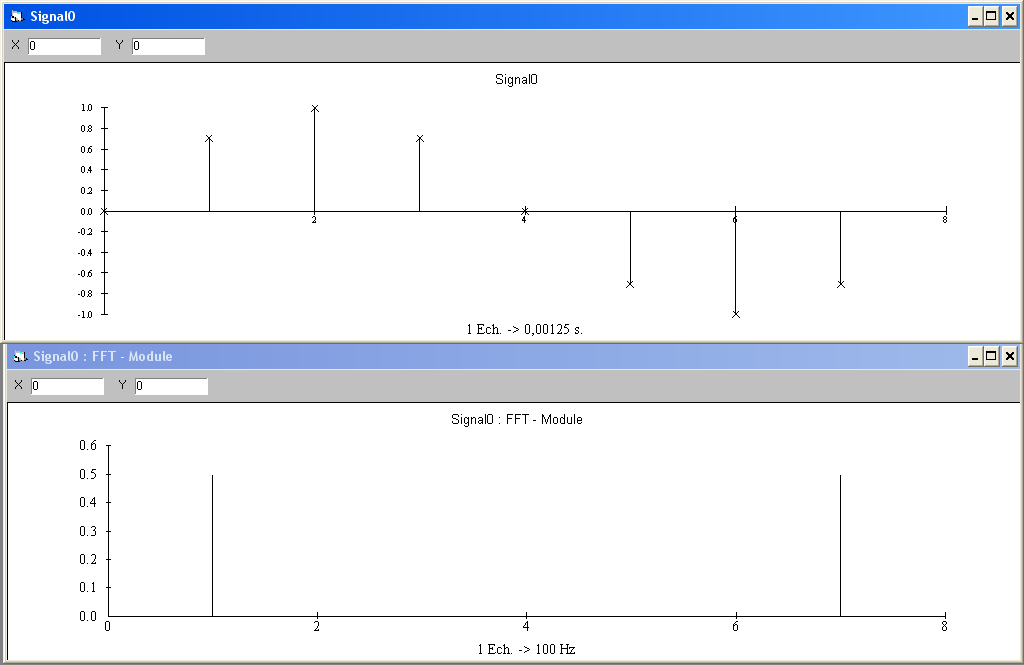
\includegraphics[width=10cm]{fig1.png}
			\caption{Allure de la transformée de Fourier}
		\end{figure}
	
		La porte est de largeur $\tau$, de période $T_{r}$  et d’amplitude A.
		Pour déterminer le spectre d’amplitude d’un signal périodique il faut passer par la série de Fourier.\\
		D’après les résultats des travaux dirigés, les coefficients de la série de Fourier sont :
		$$ A_{0} = \frac{A\tau}{T_{r}} $$
		$$ A_{n} = \frac{4 A}{T_{r}}\int_{0}^{\tau / 2} cos(n \omega t) dt = \frac{2 A \tau}{T_{r}} sinc(n \pi \frac{\tau}{T_{r}}) $$
		
		La fonction est pair donc les coefficients $B_{n}$ sont nuls. 

		Nous avons donc la série de fourier suivante : 
		
		$$ S(t) = \frac{\tau A}{T_{r}} + \sum_{1}^{+ \infty} \frac{2 A \tau}{T_{r}} sinc(n \pi \frac{\tau}{T_{r}}).cos(\frac{n 2 \pi t}{T_{r}}) $$
		
		$$ H_{1} = \frac{2 A}{\pi} sin(\frac{\pi \tau}{T_{r}}) $$
		$$ H_{2} = \frac{A}{\pi} sin(\frac{2 \pi \tau}{T_{r}}) $$
		$$ H_{3} = \frac{2A}{3 \pi} sin(\frac{3 \pi \tau}{T_{r}}) $$
		$$ H_{4} = \frac{A}{2 \pi} sin(\frac{4 \pi \tau}{T_{r}}) $$
		$$ H_{5} = \frac{2 A}{5 \pi} sin(\frac{5 \pi \tau}{T_{r}}) $$
	
	\section{Analyse de signaux harmoniques}
	
	Nous utilisons un analyseur de la marque AGILENT dont la bande spectrale pouvant être explorée est comprise entre 9 kHz et 1.5 MHz.
	
	\subsection{Réponse du filtre d'analyse}
	
	La touche CENTER FREQUENCY permet de régler la fréquence observée au milieu de l’écran.
	La touche SPAN permet de modifier la largeur de la fenêtre d’affichage.\\
	Si l’on veut mieux voir un pic ou au contraire l’atténuer, nous pouvons changer la valeur du haut de l’écran avec REF LEVEL. Ce paramètre est géré par le détecteur d’amplitude. \\
	La touche ATTÉNUATION permet d’atténuer le signal pour éviter les saturations de l’appareil, ce paramètre agit avant l’observation du signal, c’est donc l’atténuateur qui se charge de cette fonctionnalité.\\
	Pour modifier la largeur de la bande passante du filtre, nous devons utiliser la touche BW/Avg et modifier la valeur, comme son nom l’indique la largeur de la bande passante est gérée par le filtre.\\
	Enfin, la touche SWEEP permet de gérer le taux de rafraîchissement des données affichées à l’écran, ce paramètre est géré via le générateur de rampe de l’appareil.
	
	\subsection{Spectre d'un signal harmonique}
	
	Le spectre théorique d’un signal sinusoïdal est celui de la figure 1 décrit dans la préparation.\\
	En injectant avec le générateur interne, un signal de 50 MHz. Nous obtenons le résultat suivant :
	
	\begin{figure}[h]
		\centering
		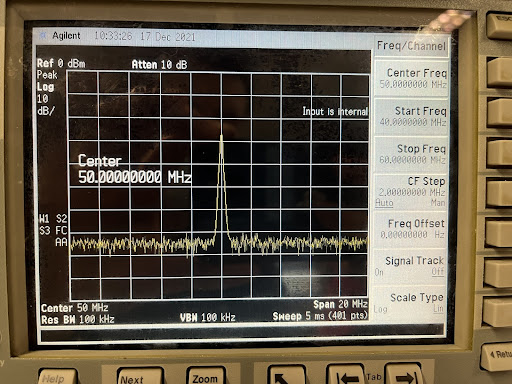
\includegraphics[width=8cm]{fig2.jpg}
		\caption{Spectre du générateur interne}
	\end{figure}
	
	Ce résultat est cohérent car avec un “span” de 20 MHz, nous ne pouvons observer qu’un seul des deux pics du spectre.\\
	C’est à partir d’une bande passante de 30 kHz,que nous pouvons considérer notre pic comme un pic de Dirac. \\
	
	\begin{figure}[h]
		\centering
		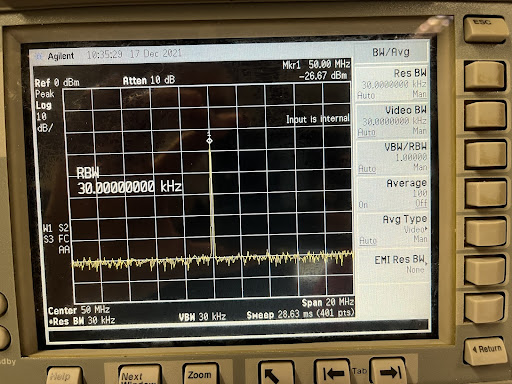
\includegraphics[width=8cm]{fig3.jpg}
		\caption{Spectre du générateur interne}
	\end{figure}
	
	Après avoir utilisé le menu MARKER, nous voyons que l’amplitude du pic vaut -26.7 dBm. Ce qui correspond bien aux données du constructeur. En modifiant, l'atténuation nous voyons que plus l’atténuation est importante, plus l’amplitude du bruit est importante aussi. Le niveau de référence est modifié, cela impacte donc le bruit interne de l’appareil. Si l'atténuation est trop forte, notre signal est noyé dans le bruit.
	
	\subsection{Spectre d'un signal modulé en amplitude}
	
	Voici le signal que nous injectons à l'oscillateur. L’amplitude crête à crête est avec 2 V et la fréquence est de 5 MHz.
	
	\begin{figure}[h]
		\centering
		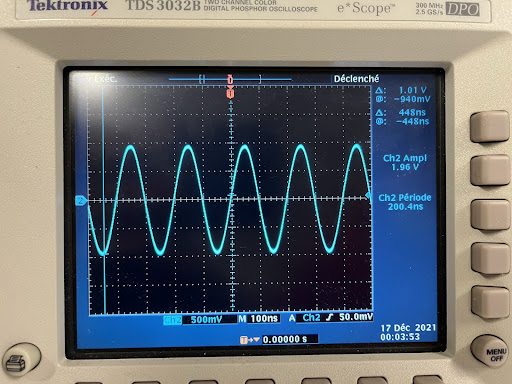
\includegraphics[width=6.5cm]{fig4.jpg}
		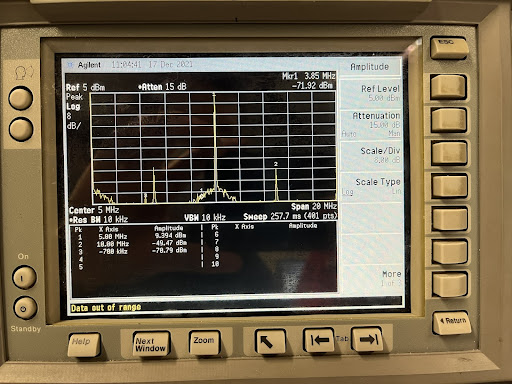
\includegraphics[width=6.5cm]{fig5.jpg}
		\caption{Spectre de la porteuse}
	\end{figure}
	
	Une fois les réglages faits, nous observons le spectre ci-dessus. Si nous augmentons le “span” nous observons des harmoniques aux multiples de la fréquence du signal. Nous pouvons donc conclure que le spectre théorique est différent du spectre pratique, le signal observé n’est pas parfait. Cependant comparé à la puissance du fondamental, la puissance des harmoniques est faible. 
	
	Nous mesurons 9.3 dBm pour l’amplitude du pic ce qui équivaut à une tension efficace de 652 mV. Nous avons une tension efficace valant 0.652 V donc la tension maximale vaut 0.92 V. En théorie, nous devrions mesurer 1.96/2 = 0.98 V. Les deux résultats sont assez proches, nous supposons que les pertes sont dues aux appareils.
	
	En ce qui concerne l’impédance de l’analyseur de spectre, la valeur change lorsque nous changeons la valeur de la résistance interne. L’appareil prends donc d’abord en compte la puissance du signal et ensuite il la calcule en fonction de la valeur de résistance choisie.\\ 
	
	Nous pouvons schématiser l’influence des résistances avec le schéma suivant.
	
	Nous avons Rg la résistance du générateur et Ras la résistance de l’analyseur de spectre, $R_{as} = R_{q} = 50\Omega$ et $ R_{0} = 50 M\Omega $ la résistance de l'oscillateur.
	Nous avons donc :
	$$ Z_{eq} = \frac{R_{as}R_{0}}{R_{as} + R_{0}} = R_{as} $$ 
	Le signal sinusoïdal valeur max $V_{1} = 1 V$\\
	$$ V_{2 max} = \frac{V_{1 max} R_{as}}{R_{as} + R_{0}} = \frac{V_{1 max}}{2} = 0.5V $$
	Nous avons donc $$ V_{2 eff} = \frac{0.5}{\sqrt{2}} = 0.35V $$
	
	Nous allons maintenant injecter un signal modulé AM dans l’analyseur de spectre. La porteuse est reglée à 5 Mhz et le signal à transmettre est de 2kHz et a une amplitude crête de 100 mV.
	
	\begin{figure}[h]
		\centering
		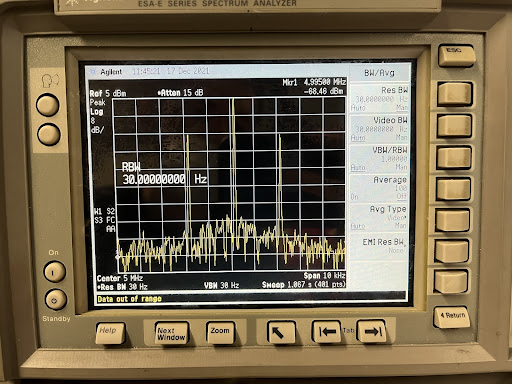
\includegraphics[width=11cm]{fig6.jpg}
		\caption{Spectre signal modulé}
	\end{figure}
	
	Nous avons un span de 10 kHz et 10 carreaux affichés à l’écran donc 1 carreaux à une largeur d’1 kHz, les pics sont donc bien espacés de 2 kHz, c’est le résultat que nous attendons. 
	Ce spectre est bien le spectre attendu.\\
	
	Comparons maintenant leur amplitude avec la théorie.
	
	
\end{document}